% !TEX root = ../macro.tex
\section{Ramsey Model}\label{sec:ramsey}

Solow determines accumulation from a given saving share. Ramsey asks how much
to consume and save when households value consumption at different dates.
The change adds a choice, a price for postponing consumption, and a boundary
condition that selects an admissible path.

\subsection{From a saving rule to a saving decision}

Suppose two economies have the same current income. In one, income is expected
to rise; in the other, a disruption has temporarily reduced production. A rule
$S=sY$ makes saving move proportionally with current output in both cases.
It cannot tell us whether households want to smooth a temporary loss, prepare
for lower future income, or invest in a newly productive opportunity.

One response would be to make $s$ a function of income or the interest rate.
But then we would still need to explain that function and how it changes when
expectations or policy change. Instead, specify what consumption is worth,
what saving buys, and which paths the household can finance. A saving rate
will emerge from those choices rather than being the starting rule.

Start with the experiment of consuming one unit less today. Saving that unit
provides a return tomorrow. The household compares the utility lost now with
the discounted utility of that future consumption. This suggests an optimality
condition across adjacent dates. It cannot yet determine the level of
consumption: a household with little wealth cannot finance every path with
the right slope. We will need feasibility and a terminal restriction as well.

The planner and household formulations then answer related questions. The
planner allocates real resources; a household takes wages and returns as given.
Their allocations coincide in the competitive benchmark under the conditions
stated below. Taxes can separate the private return from the social product,
which is why decentralization matters for the final section.

Ramsey's original contribution was a saving problem; the presentation here is
the modern discounted Ramsey--Cass--Koopmans benchmark, rather than a literal
reproduction of the 1928 objective.\footnote{Frank P. Ramsey (1928), ``A
Mathematical Theory of Saving,'' \textit{Economic Journal}, 38(152), 543--559.
\url{https://doi.org/10.2307/2224098}.}

% BEGIN ORIGINAL COURSE ASSUMPTIONS - retained, not typeset
% \subsection{Assumptions}\label{assumptions}
% 
% 
% 
% \begin{itemize}
%   \item Same as Solow Model
%     \begin{itemize}
%     \tightlist
%       \item Production Function in the Harrold neutrality form
%       \item \textbf{Exogenous Variables:}
%       \item Population growth rate$=n$
%       \item Technology growth rate$=g$
%       \item Depreciation rate$=0$ (for simplicity)
%       \item And most of all, the technological growth rate is assumed as $a$.
%     \end{itemize}
%   \item Firm
%     \begin{itemize}
%     \tightlist
%       \item Perfect competitive firms, or homogenous firms, or representive firms
%       \item Hire workers and capital in competitive factor markets
%       \item Each has the production function $Y=F(K,AL)$
%       \item Firms are owned by the families, meaning the revenue goes straight to
%       latter
%     \end{itemize}
%   \item Household
%     \begin{itemize}
%     \tightlist
%       \item Homogenous families.
%       \item Population growth of each household is assumed as $n$.
%       \item Each member in a household provides one unit of labor.
%       \item Income of a household is the sum of the labor revenue subsum, the capital revenue subsum and the firm revenue share subsum.
%       \item A household should and must maximize the utility.
%       \item Degree of patience denoted as discount factor $\beta=\frac{1}{1+\rho}$, and $\rho$ is the discount rate.
%     \end{itemize}
% \end{itemize}
% 
% 
% 
% \begin{blueblock}
% \begin{note}[Rule of Prohibiting Ponzi Schemes]
% Conconstraint in Ramsey model is also called Prohibiting Ponzi Schemes Rule. It forbids the household to do a scam of rolling over debt by repeatedly borrowing. Yet in real life, many people are doing this as a harmless way to ralex debt pressure.
% \end{note}
% \end{blueblock}
% 
% END ORIGINAL COURSE ASSUMPTIONS

\Needspace{34\baselineskip}
\subsection{Assumptions}\label{assumptions}

The economic environment follows Solow. The new ingredient is a household
objective, so the map separates its choices from technology and market clearing.

\begin{modelsetup}
\begin{modelcondition}{01}{Technology and resources}
A closed, one-good economy without government in the baseline:
\[
Y=F(K,AL),\quad Y=C+I.
\]
Production has the Solow properties.
\end{modelcondition}
\begin{modelcondition}{02}{Given states and paths}
Positive initial stocks. Labor and technology grow exogenously:
\[
\dot L/L=n,\qquad \dot A/A=g.
\]
The course benchmark sets $\delta=0$.
\end{modelcondition}
\begin{modelcondition}{03}{Households}
Identical, price-taking dynasties own capital. Each member supplies one unit
of labor and chooses consumption over time.
\end{modelcondition}
\begin{modelcondition}{04}{Preferences}
Utility is defined over consumption per person, $x=C/L$:
\[
\int_0^\infty e^{-\rho t}L(t)u(x(t))\,dt.
\]
Patience and curvature affect saving.
\end{modelcondition}
\begin{modelcondition}{05}{Firms and prices}
Competitive firms maximize profits. Rental income and wages go to households;
profits are zero under constant returns.
\end{modelcondition}
\begin{modelcondition}{06}{Feasible optimal paths}
Capital is inherited; consumption is chosen. Feasibility, optimality, market
clearing, and terminal conditions jointly select a path.
\end{modelcondition}
\end{modelsetup}

\subsubsection{Notation and the course simplifications}

Use $K,C,Y$ for aggregates and $x=C/L$ for consumption per person. Reserve
$k=K/(AL)$ and $c=C/(AL)$ for quantities per effective worker, so $x=Ac$.
Technology growth is denoted by $g$ throughout. We retain the course's
zero-depreciation benchmark; $\delta$ remains visible in the formulas so that
setting $\delta=0$ is explicit. Full depreciation, $\delta=1$, will be used
only in a separately labeled discrete-time example.

Preferences have marginal utility $u'(x)=x^{-\theta}$, $\theta>0$:
\begin{equation}\label{eq:ramsey-utility}
u(x)=\begin{cases}
 x^{1-\theta}/(1-\theta),&\theta\ne1,\\
 \log x,&\theta=1.
\end{cases}
\end{equation}
In this deterministic model, $1/\theta$ measures willingness to substitute
consumption across time. Higher $\rho$ reduces the weight on future utility.
Assume $\rho>n\geq0$, $g\geq0$, and
\begin{equation}\label{eq:ramsey-effective-discount}
\eta\equiv\rho-n-(1-\theta)g>0.
\end{equation}
These are sufficient restrictions for finite utility on the balanced growth
path used below. Weighting by $L(t)$ means the dynasty values the utility of
all its members; choosing a different population welfare criterion would change
the normalization. The original lists are retained in comments immediately
above this section for comparison.

\subsubsection{No-Ponzi restrictions and transversality}

A household's total wealth $B$ satisfies
\begin{equation}
\dot B=rB+wL-C,
\end{equation}
where $r$ is the net real return and $w$ the wage per person. A no-Ponzi
restriction requires
\begin{equation}\label{eq:ramsey-npg}
\liminf_{T\to\infty}e^{-\int_0^T r(v)\,dv}B(T)\geq0.
\end{equation}
Borrowing must ultimately be supported by resources rather than by a negative
terminal present value of wealth. Refinancing a loan is not, by itself, a
Ponzi scheme: future income can support repayment.

A transversality condition instead concerns optimality. In the planner's
normalized problem below it takes the standard form
\begin{equation}\label{eq:ramsey-tvc}
\lim_{t\to\infty}e^{-\eta t}u'(c(t))k(t)=0.
\end{equation}
It rules out leaving resources with positive limiting discounted utility value
when consuming more would improve the allocation. It does not require the
capital stock itself to approach zero. Feasibility and an Euler equation alone
need not select the optimal infinite-horizon path.

\subsection{Solving the consumption--saving problem}

\subsubsection{The planner's problem and decentralization}\label{central-planners-problem}

For continuous time, the planner chooses consumption with inherited $K(0)$:
\begin{equation}\label{eq:ramsey-planner}
\begin{split}
\max_{\{C(t)\}}\;&\int_0^\infty e^{-\rho t}L(t)u(C(t)/L(t))\,dt,\\
\text{s.t. }&\dot K=F(K,AL)-\delta K-C,\qquad K\geq0,\ C>0.
\end{split}
\end{equation}
Consumption uses current output; the residual, net of depreciation, changes
the capital stock. In a decentralized economy, a household uses its budget
constraint instead. Competitive factor pricing gives
\begin{equation}\label{eq:ramsey-factor-prices}
q=f'(k),\qquad r=q-\delta,\qquad
w=A\left[f(k)-kf'(k)\right].
\end{equation}
$q$ is the rental payment before depreciation. The net return $r=q-\delta$
and a discrete-time gross return $R=1+q-\delta=1+r$ are different objects.

With constant returns, factor incomes exhaust output. Firms' dividends are
not an additional source of aggregate goods on top of $Y$. In equilibrium,
aggregate household wealth equals capital, $B=K$, so the household budgets
consolidate into \eqref{eq:ramsey-planner}'s resource constraint. With identical
preferences, competitive prices, and no taxes, externalities, or financing
frictions, the planner allocation can be supported as a competitive allocation.
This equivalence must be checked again when the environment changes.

\subsubsection{Lagrangian: the adjacent-date trade-off}\label{method-of-lagrangian}

First isolate discrete time with $A=L=1$ and $n=g=0$. This makes timing visible
without carrying growing denominators; it is a restricted version of the model.
The planner solves
\begin{equation}
\max_{\{c_t,k_{t+1}\}}\sum_{t=0}^\infty\beta^tu(c_t),\qquad
c_t+k_{t+1}=f(k_t)+(1-\delta)k_t,
\end{equation}
where $k_0$ is given, $0<\beta<1$, and $0\leq\delta\leq1$. Writing
$\beta=1/(1+\rho)$ defines a discrete-time rate of time preference; the
continuous-time convention uses $e^{-\rho t}$.

Use current-utility multipliers $\lambda_t$:
\begin{equation}
\mathscr L=\sum_{t=0}^\infty\beta^t
\left\{u(c_t)+\lambda_t[f(k_t)+(1-\delta)k_t-c_t-k_{t+1}]\right\}.
\end{equation}
At an interior solution, differentiate with respect to $c_t$ and $k_{t+1}$:
\begin{align}
\lambda_t&=u'(c_t),\\
\lambda_t&=\beta\lambda_{t+1}[f'(k_{t+1})+1-\delta].
\end{align}
Substitution gives the Euler equation
\begin{equation}\label{eq:ramsey-discrete-euler}
u'(c_t)=\beta R_{t+1}u'(c_{t+1}),\qquad
R_{t+1}=f'(k_{t+1})+1-\delta.
\end{equation}
One unit saved at $t$ earns its return at $t+1$, when the new capital is used.
The utility cost today equals the discounted marginal gain tomorrow. For CRRA,
\begin{equation}
\frac{c_{t+1}}{c_t}=(\beta R_{t+1})^{1/\theta}.
\end{equation}
This determines consumption growth given the return, not the entire consumption
path. With no bequest motive and the usual concavity conditions, the terminal
condition is $\lim_{t\to\infty}\beta^tu'(c_t)k_{t+1}=0$. In a finite-horizon
exercise a terminal stock may be set to zero; that is not the same as imposing
$k_t\to0$ in this infinite-horizon economy.

\subsubsection{Hamiltonian: saving with continuous adjustment}\label{method-of-hamiltonian-equation-optimal-control}

Return to continuous time with population and technology growth. From
$k=K/(AL)$ and $c=C/(AL)$,
\begin{equation}\label{eq:ramsey-capital-motion}
\dot k=f(k)-c-bk,\qquad b\equiv n+g+\delta.
\end{equation}
For $\theta\ne1$, substitute $x=Ac$ and $L=L_0e^{nt}$ into utility:
\begin{equation}
e^{-\rho t}Lu(Ac)
=L_0A_0^{1-\theta}e^{-\eta t}\frac{c^{1-\theta}}{1-\theta}.
\end{equation}
The positive constant in front does not change choices. For log utility,
$\log(Ac)=\log A+\log c$; the $\log A$ term is independent of the allocation.
The normalized problem therefore discounts $u(c)$ at $\eta$ in either case.

Its current-value Hamiltonian is
\begin{equation}
\mathcal H=u(c)+\mu[f(k)-c-bk].
\end{equation}
The control condition and current-value costate equation are
\begin{align}
\mathcal H_c=0&\quad\Longrightarrow\quad \mu=u'(c),\\
\dot\mu=\eta\mu-\mathcal H_k
&=\left[\eta+b-f'(k)\right]\mu.
\end{align}
$\mu$ is the current utility value of an additional unit of normalized capital.
The factor $\eta$ belongs in the current-value costate equation; a
present-value costate would instead absorb the discount factor. These are two
representations of the same problem, not an assertion that patience is irrelevant.

Differentiate $\mu=c^{-\theta}$ and use
$\eta+b=\rho+\delta+\theta g$:
\begin{align}
\frac{\dot\mu}{\mu}&=-\theta\frac{\dot c}{c}
 =\eta+b-f'(k),\\
\frac{\dot c}{c}
&=\frac{f'(k)-\delta-\rho-\theta g}{\theta}.
\label{eq:ramsey-normalized-euler}
\end{align}
Consumption per person is $x=Ac$, so
\begin{equation}\label{eq:ramsey-person-euler}
\frac{\dot x}{x}=g+\frac{\dot c}{c}
 =\frac{r-\rho}{\theta}.
\end{equation}
A high return makes future consumption relatively attractive; impatience favors
consumption now. Curvature determines how strongly consumption growth responds.
Population growth affects resources and welfare weights, but cancels from this
per-person Euler equation under the dynasty objective specified above.

Setting $\delta=0$ recovers the course benchmark. Setting $g=n=0$ also removes
the growth normalization. At $\rho=0$ the intertemporal trade-off changes, and
an infinite-horizon undiscounted problem needs its own welfare criterion; it is
not obtained simply by deleting discounting from every infinite integral.

\subsubsection{Bellman and HJB: valuing the remaining opportunities}\label{method-of-bellman-equation-dynamic-programming}

For the stationary discrete-time version, let $V(k)$ be the value of starting
with capital $k$. Choose next period's capital $k'$:
\begin{equation}
V(k)=\max_{k'}\left\{u(f(k)+(1-\delta)k-k')+\beta V(k')\right\},
\end{equation}
with feasible $k'\geq0$ and positive current consumption. At an interior optimum,
\begin{align}
u'(c)&=\beta V'(k'),\\
V'(k)&=u'(c)[f'(k)+1-\delta].
\end{align}
The second line is the envelope condition: the effect of the optimal choice's
response drops out at the optimum. Apply it at $k'$ in the first line to recover
\eqref{eq:ramsey-discrete-euler}. The Lagrangian and Bellman methods are pricing
the same marginal transfer of resources between dates.

\textbf{A case with an exact saving rule.}
Take $u(c)=\log c$, $f(k)=k^\alpha$, and full depreciation $\delta=1$ only for
this example. Guess $V(k)=a+d\log k$. The first-order condition gives
\begin{equation}
\frac{1}{k^\alpha-k'}=\frac{\beta d}{k'},\qquad
\frac{k'}{k^\alpha}=\frac{\beta d}{1+\beta d}.
\end{equation}
Matching the coefficient of $\log k$ in the Bellman equation yields
$d=\alpha(1+\beta d)$, hence
\begin{equation}\label{eq:ramsey-exact-saving}
d=\frac{\alpha}{1-\alpha\beta},\qquad
k'=\alpha\beta k^\alpha,\qquad c=(1-\alpha\beta)k^\alpha.
\end{equation}
A constant saving share can emerge from optimization in this special case. Its
value depends on preferences and technology; the result does not make a
constant saving share general once depreciation or utility changes.

In normalized continuous time, dynamic programming gives the HJB equation
\begin{equation}
\eta V(k)=\max_c\{u(c)+V'(k)[f(k)-c-bk]\}.
\end{equation}
The control condition is $u'(c)=V'(k)$. Differentiate using the envelope theorem:
\begin{equation}
\eta V'(k)=V''(k)\dot k+V'(k)[f'(k)-b].
\end{equation}
Along the path, $\dot\mu=V''(k)\dot k$ with $\mu=V'(k)$, giving the same
costate equation and consumption Euler equation as the Hamiltonian. The value
function summarizes all future opportunities; the terminal and feasibility
conditions remain part of the underlying problem.

\subsection{Intertemporal equilibrium and economic adjustment}

\subsubsection{Steady state and the two loci}

The continuous-time equilibrium combines
\begin{equation}\label{eq:ramsey-system}
\begin{split}
\dot k&=f(k)-c-bk,\\
\dot c&=\frac{c}{\theta}[f'(k)-\delta-\rho-\theta g],
\end{split}
\end{equation}
with given $k(0)$ and \eqref{eq:ramsey-tvc}. A positive normalized steady state
satisfies
\begin{equation}\label{eq:ramsey-steady}
f'(k^*)=\delta+\rho+\theta g,\qquad c^*=f(k^*)-bk^*.
\end{equation}
The production assumptions give a unique positive $k^*$. Strict concavity gives
$f(k^*)/k^*>f'(k^*)>b$, where the second inequality is $\eta>0$, so $c^*>0$.
On this balanced growth path, consumption per person grows at $g$, aggregate
consumption at $n+g$, and the net return is $r^*=\rho+\theta g$.

For $c>0$, the $\dot c=0$ locus is vertical at $k^*$. Consumption grows to its
left and falls to its right. The $\dot k=0$ locus is $c=f(k)-bk$; capital grows
below it and falls above it. If $b>0$, its maximum is the Golden Rule stock,
where $f'(k_{\mathrm{GR}})=b$. Neither locus, by itself, is an equilibrium path.

\begin{center}
\begin{minipage}{\linewidth}
\centering
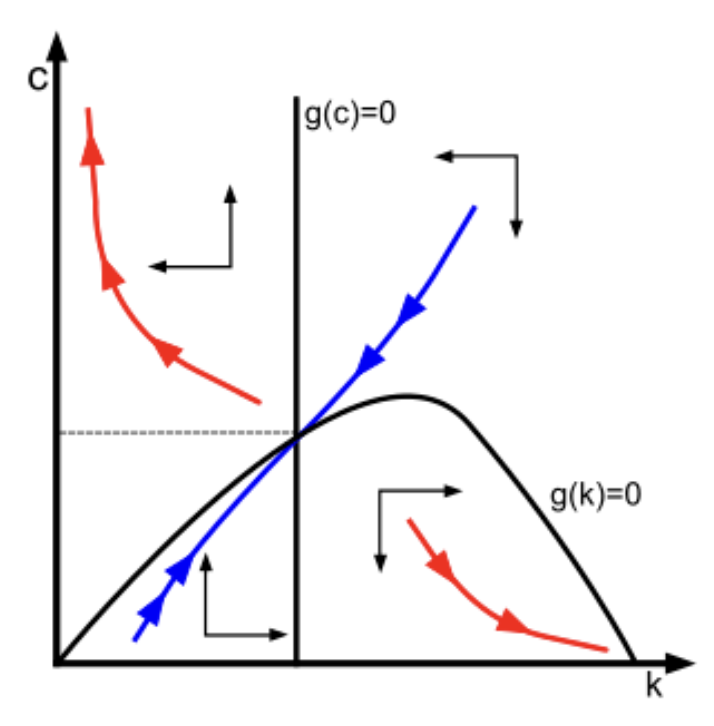
\includegraphics[width=0.48\linewidth]{images/ramsey_phase_diagram.png}
\par\medskip\RaggedRight
\noindent\textit{Reading the diagram.} The vertical line is $\dot c=0$; the
curved resource locus is $\dot k=0$. The blue curve depicts the stable path,
with arrows toward their intersection. The red paths illustrate departures
that do not satisfy the required long-run conditions. The sketch assumes a
hump-shaped resource locus and $k^*<k_{\mathrm{GR}}$.
\end{minipage}
\end{center}

\subsubsection{Why consumption can jump while capital cannot}

Capital is a state inherited from previous investment. Consumption is a control:
a household can change spending immediately, but cannot instantly create a
new stock of machines. For a given $k(0)$, different initial consumption choices
produce different candidate paths under \eqref{eq:ramsey-system}. Most fail
feasibility or the terminal condition. The saddle path selects initial
consumption as well as the later transition; it does not require every variable
to start at its steady state.

A one-time destruction of physical capital, with all other fundamentals
unchanged, moves the state leftward. Consumption adjusts onto the stable path.
The low stock supports a high return and rebuilding, while the loss of resources
constrains current spending. Actual disasters may also damage skills or
technology, which would change the destination rather than just the initial state.

A credible announcement about future productivity or taxation can change
consumption before it changes current output: the household evaluates future
income and returns when choosing today's spending. This model isolates that
intertemporal mechanism. It omits borrowing constraints, income risk, and
different marginal propensities to consume, so its representative consumption
response is not an empirical claim about every household.

\subsection{Linearization and the saddle path}

\subsubsection{The local system and its eigenvalues}

Let $\Delta k=k-k^*$ and $\Delta c=c-c^*$. In the order $(k,c)$, the first-order
system is
\begin{equation}\label{eq:ramsey-jacobian}
\begin{pmatrix}\dot{\Delta k}\\\dot{\Delta c}\end{pmatrix}
\approx
J\begin{pmatrix}\Delta k\\\Delta c\end{pmatrix},\qquad
J=\begin{pmatrix}\eta&-1\\ z&0\end{pmatrix},\quad
z\equiv\frac{c^*f''(k^*)}{\theta}<0.
\end{equation}
The top-left entry is $f'(k^*)-b=\eta$; the bottom-right entry vanishes because
the consumption growth bracket is zero at the steady state. Thus
\begin{equation}
\det(\lambda I-J)=\lambda^2-\eta\lambda+z=0,\qquad
\lambda_{\pm}=\frac{\eta\pm\sqrt{\eta^2-4z}}{2}.
\end{equation}
Since $z<0$, $\lambda_-<0<\lambda_+$. The local system has one stable and one
unstable direction. This is the mathematical reason a boundary condition is
needed to select consumption for the inherited capital stock.

For a stable eigenvector $(1,m)$, the first row implies
$m=\eta-\lambda_->0$. The local stable path is therefore
\begin{align}
\Delta c(0)&\approx m\Delta k(0),\\
\Delta k(t)&\approx\Delta k(0)e^{\lambda_-t},\\
\Delta c(t)&\approx m\Delta k(0)e^{\lambda_-t}.
\end{align}
The positive convergence speed is $-\lambda_-$; its local half-life is
$\log2/(-\lambda_-)$. The exponential solution is exact for the linearized
system, and generally approximate for the original nonlinear transition.

\subsubsection{The same restriction by undetermined coefficients}

Alternatively, conjecture a local policy $\Delta c=m\Delta k$. From the first
linearized equation, $\dot{\Delta k}=(\eta-m)\Delta k$. Differentiating the
conjecture and using the second equation gives
\begin{equation}
m(\eta-m)\Delta k=z\Delta k,\qquad m^2-\eta m+z=0.
\end{equation}
Choose the positive root $m=\lambda_+$, so $\eta-m=\lambda_-<0$. This recovers
the same stable policy. Choosing the decaying direction is not a free change
to initial capital; it is the restriction on the consumption choice implied
by admissibility and optimality.

\subsection{Maximizing welfare}\label{maximizing-welfare}

Similiar to the concept of golden rate in Solow model, Ramsey model also provide a glimpse of maximized consumption.

At the steady state
\begin{align}
&c^{*}= F(k^{*})-\delta k^{*}
\\&\Rightarrow k^*_{gold}=\underset{k^*}{\text{argmax}} \;c^{*}
\end{align}











\subsection[Taxation and capital accumulation (planned)]{Taxation and capital accumulation}
\textit{Planned section.} Compare lump-sum and distortionary taxes in the neoclassical growth framework.
Separate effects on steady-state capital from effects along the transition.
